% !TEX program = xelatex
\documentclass[11pt,a4paper]{article}
\newcommand{\DOCFOOT}{AMPERE POINT · Q11 z modułem Shelly X · dokumentacja testów v1 · 28 września 2026}
% Wspólna preambuła dokumentów dla producenta (xelatex); kopia z raportu DLB, czcionki systemowe Windows
\usepackage{fontspec}
% \ZHDOC zdefiniowane przed \input => cały dokument po chińsku (Noto Sans CJK SC + łamanie wierszy CJK)
\ifdefined\ZHDOC
  \setmainfont{Microsoft YaHei}[Scale=0.90]
  \setsansfont{Microsoft YaHei}[Scale=0.90]
  \XeTeXlinebreaklocale "zh"
  \XeTeXlinebreakskip = 0pt plus 1pt minus 0.1pt
\else
  \setmainfont{Calibri}
  \setsansfont{Calibri}
\fi
\setmonofont{Consolas}[Scale=0.86]
\newfontfamily\cjkfont{Microsoft YaHei}[Scale=0.90]
\newfontfamily\latinfont{Calibri}
\newcommand{\pl}[1]{{\latinfont #1}}
\usepackage[a4paper,top=2.0cm,bottom=2.0cm,left=1.9cm,right=1.9cm]{geometry}
\usepackage{graphicx}
\usepackage[table]{xcolor}
\usepackage{booktabs,longtable,array,tabularx,enumitem,fancyhdr,caption}
\usepackage[most]{tcolorbox}
\usepackage[hidelinks,unicode]{hyperref}
\usepackage{needspace}
\usepackage{float}
\emergencystretch=2.5em
\setlength{\parindent}{0pt}\setlength{\parskip}{5pt}
\renewcommand{\arraystretch}{1.22}
\captionsetup{font=small,labelfont=bf,skip=3pt}
\setlist{nosep,leftmargin=*}
\setcounter{secnumdepth}{2}

\definecolor{apnavy}{HTML}{1A1A1A}
\definecolor{apink}{HTML}{1C2430}
\definecolor{apmuted}{HTML}{5B6675}
\definecolor{apline}{HTML}{E3E3E3}
\definecolor{apbg}{HTML}{F5F5F5}
\definecolor{apaccent}{HTML}{EC6434}
\definecolor{apaccentbg}{HTML}{FDEDE6}
\definecolor{apwarn}{HTML}{B9791B}
\definecolor{apwarnbg}{HTML}{FBF1DE}
\definecolor{apred}{HTML}{B91C1C}
\definecolor{apredbg}{HTML}{FEE2E2}
\definecolor{apgreen}{HTML}{1F8A4C}
\definecolor{apgreenbg}{HTML}{E7F5EC}
\definecolor{aphead}{HTML}{EDEDED}

\pagestyle{fancy}\fancyhf{}
\renewcommand{\headrulewidth}{0pt}
\fancyfoot[L]{\footnotesize\color{apmuted}\DOCFOOT}
\fancyfoot[R]{\footnotesize\color{apmuted}\thepage\,/\,\pageref{LastPage}}
\usepackage{lastpage}

\usepackage{titlesec}
\titleformat{\section}{\Large\bfseries\color{apnavy}}{\thesection}{0.6em}{}
\titlespacing*{\section}{0pt}{14pt}{6pt}
\titleformat{\subsection}{\large\bfseries\color{apnavy}}{\thesubsection}{0.6em}{}
\titlespacing*{\subsection}{0pt}{10pt}{4pt}

% pasek tytułowy
\newcommand{\apheader}[3]{%
\noindent
\includegraphics[height=1.0cm]{logo_ap.png}\hfill
\raisebox{0.25cm}{\parbox[t]{10.5cm}{\raggedleft\footnotesize\color{apmuted}#3}}\\[0.25cm]
{\color{apaccent}\rule{\textwidth}{1.8pt}}\\[0.30cm]
{\bfseries\color{apnavy}\LARGE #1}\\[0.18cm]
{\large\color{apmuted}#2}\\[0.2cm]}

% ramki
\newtcolorbox{apbox}[1][]{enhanced,breakable,colback=apbg,colframe=apline,boxrule=0.6pt,arc=3pt,left=7pt,right=7pt,top=5pt,bottom=5pt,fonttitle=\bfseries,coltitle=apnavy,colbacktitle=aphead,title={#1}}
\newtcolorbox{apwarnb}[1][]{enhanced,breakable,colback=apwarnbg,colframe=apwarn,boxrule=0.6pt,arc=3pt,left=7pt,right=7pt,top=5pt,bottom=5pt,fonttitle=\bfseries,title={#1}}
\newtcolorbox{apredb}[1][]{enhanced,breakable,colback=apredbg,colframe=apred,boxrule=0.6pt,arc=3pt,left=7pt,right=7pt,top=5pt,bottom=5pt,fonttitle=\bfseries,title={#1}}
\newtcolorbox{apgreenb}[1][]{enhanced,breakable,colback=apgreenbg,colframe=apgreen,boxrule=0.6pt,arc=3pt,left=7pt,right=7pt,top=5pt,bottom=5pt,fonttitle=\bfseries,title={#1}}

% komórka ze zrzutem ekranu: #1 szerokość, #2 plik, #3 podpis
\newcommand{\shot}[3]{%
\begin{minipage}[t]{#1}
  \vspace{0pt}\centering
  \includegraphics[width=\linewidth,height=6.2cm,keepaspectratio]{#2}\par\vspace{3pt}
  {\footnotesize\color{apink}#3\par}
\end{minipage}}


% mniejsza komórka ze zdjęciem (np. gniazda aut)
\newcommand{\shotsm}[3]{%
\begin{minipage}[t]{#1}
  \vspace{0pt}\centering
  \includegraphics[width=\linewidth,height=4.6cm,keepaspectratio]{#2}\par\vspace{3pt}
  {\footnotesize\color{apink}#3\par}
\end{minipage}}

\newcommand{\kroknum}[1]{{\colorbox{apaccent}{\textcolor{white}{\bfseries\small\,#1\,}}}}
\newcommand{\dpn}[1]{{\cjkfont #1}}
\newcommand{\Fact}{\textcolor{apgreen}{\textbf{[fact]}}}
\newcommand{\Hyp}{\textcolor{apwarn}{\textbf{[hypothesis]}}}

\setlength{\tabcolsep}{4pt}
\renewcommand{\figurename}{Rysunek}
\newfontfamily\symbolfont{Segoe UI Symbol}
\newcommand{\ok}{{\symbolfont\color{apgreen}\textbf{✔}}}
\newcommand{\half}{{\symbolfont\color{apwarn}\textbf{◐}}}
\newcommand{\no}{{\symbolfont\color{apred}\textbf{✘}}}
\newcommand{\ra}{{\symbolfont →}}
\newcommand{\la}{{\symbolfont ←}}
\newcommand{\hx}[1]{\texttt{#1}}
\hypersetup{pdftitle={Ładowarka Q11 z modułem Shelly X: dokumentacja testów i mapowanie interfejsu},pdfauthor={AMPERE POINT}}
\begin{document}

\apheader{Ładowarka Q11 z modułem Shelly X}%
{Dokumentacja testów i mapowanie interfejsu: połączenie, protokół szeregowy, punkty danych, wyniki, pytania otwarte}%
{AMPERE POINT — R\&D · dokumentacja dla producenta\\28 września 2026 · wersja 1\\Opracował Dawid Cekała}

{\small\color{apmuted}Wersja polska dokumentu wysłanego producentowi po angielsku i chińsku; treść identyczna.}

\section{Cel i zakres}

AmperePoint sprawdza możliwość zastąpienia modułu Wi-Fi Tuya WBR3 w ładowarce Q11 (produkt fabryczny \texttt{Q21\_11kW\_with\_OTA}, płytka sterująca \texttt{X2Q322\_K\_V4}) modułem Shelly X. Dokument zapisuje, co sprawdzono na prawdziwej Q11 między 24 a 28 września 2026: jak moduł jest podłączony, co sterownik wysyła po łączu szeregowym, jak są mapowane jego punkty danych, które próby się powiodły i jakie pytania pozostają otwarte. Adresatem są inżynierowie działu rozwoju producenta.

\begin{apgreenb}[Wynik w jednym zdaniu]
Sterownik Q11 pracuje z modułem Shelly \textbf{bez żadnej zmiany w oprogramowaniu sterownika}. Moduł Shelly mówi protokołem szeregowym Tuya MCU przy 9600~b/s; wystarczają cztery połączenia (3,3~V, GND, RXD, TXD). Włączanie ładowania, limit prądu, stan pracy, stan połączenia, temperatura, dane faz i bity błędów były wymieniane w obie strony przez około dziesięć godzin logu na poziomie ramek 25 września 2026 (10:51--20:48).
\end{apgreenb}

\begin{longtable}{>{\raggedright\arraybackslash}p{3.2cm}>{\raggedright\arraybackslash}p{12.9cm}}
\toprule
\rowcolor{aphead}\textbf{W zakresie} & \textbf{Szczegóły} \\
\midrule\endhead
\bottomrule\endfoot
Sprzęt & miejsce U10, pola faktycznie używane przez płytkę, nóżki sterownika, zasilanie modułu z płytki \\
Łącze szeregowe & protokół Tuya MCU zaobserwowany na przewodzie: sekwencja startowa, ruch rutynowy, zachowanie przy zapisie, przykładowe ramki \\
Punkty danych & wszystkie 17 punktów danych z definicji produktu: typ, kodowanie, czy sterownik je zgłasza, jak są mapowane w produkcie Shelly \\
Testy & sterowanie i stan w obie strony, praca bez chmury, dostarczanie czasu, lokalna warstwa integracji (krótko) \\
\rowcolor{aphead}\textbf{Poza zakresem} & \\
Chmura i aplikacja & chmura Shelly, ekrany aplikacji Shelly i zaplecze AmperePoint nie są tu opisane; nic w nich nie wymaga niczego od sterownika \\
\end{longtable}

\section{Sprzęt}

\begin{longtable}{>{\raggedright\arraybackslash}p{3.2cm}>{\raggedright\arraybackslash}p{12.9cm}}
\toprule
\rowcolor{aphead}\textbf{Element} & \textbf{Szczegóły} \\
\midrule\endhead
\bottomrule\endfoot
Ładowarka & AmperePoint Q11, przenośna, trójfazowa, 11~kW. Płytka sterująca \texttt{X2Q322\_K\_V4} (260703). Sterownik: mikrokontroler LQFP64 z naklejką \emph{„X2Q311OW OTA V22”}. Moduł Tuya WBR3 wylutowany z miejsca U10. \\
Moduł prototypowy & Shelly DevKit M1 v1.1 (płytka referencyjna Espressif) z modułem Shelly-X-MOD1-H8 (rdzeń ESP32-C3, oprogramowanie Shelly \texttt{2.0.0-beta11}), rys.~\ref{fig:devkit}. Połączony z U10 czterema przewodami i zasilany z płytki. \\
Moduł docelowy & Shelly X module X1, sprzęt V020, karta katalogowa wersja 14 (w załączniku). Ten sam obrys co WBR3: 16~$\times$~24~mm, 2~$\times$~8 pól, raster 2~mm. \\
Konfiguracja produktu Shelly & utworzona w portalu deweloperskim Shelly X: źródło danych „Tuya MCU” na IO4 (TX) / IO5 (RX), 9600~b/s, 7 zadeklarowanych punktów danych, 6 pól (stan, limit prądu, tryb, dane faz, energia sesji, czas sesji), skrypt usługi v3 napisany przez AmperePoint. \\
Narzędzia & multimetr (ciągłość i test diod na wszystkich 16 polach), dziennik diagnostyczny modułu czytany przez Wi-Fi (poziom ramek, każda ramka szeregowa ze znacznikiem czasu), narzędzia w Pythonie do testów MQTT i OCPP. \\
\end{longtable}

\begin{figure}[H]
\centering
\shot{0.46\textwidth}{devkit_top.jpg}{Shelly DevKit M1, góra: USB-C, most USB--UART, dioda RGB, moduł Shelly-X-MOD1-H8 z anteną}\hspace{0.6cm}
\shot{0.46\textwidth}{devkit_bottom.jpg}{Spód: opisy nóżek. Nóżki 4 i 5 (TX, RX) idą do Q11; nóżki z napisami RX/TX to port USB i logu, nieużywane}
\caption{Moduł prototypowy użyty w testach.}
\label{fig:devkit}
\end{figure}

\section{Połączenie elektryczne}

\subsection{Miejsce U10: co płytka faktycznie używa}

Pomiar przy wyłączonej ładowarce, test diod, czerwony przewód na polu GND. Wynik: \textbf{tylko cztery pola mają jakiekolwiek połączenie ze sterownikiem}. Wszystkie pozostałe pokazują przerwę (OL) do GND, do VCC i między sobą.

\begin{longtable}{>{\raggedright\arraybackslash}p{0.8cm}>{\raggedright\arraybackslash}p{1.6cm}>{\raggedright\arraybackslash}p{4.3cm}>{\raggedright\arraybackslash}p{4.3cm}>{\raggedright\arraybackslash}p{4.2cm}}
\toprule
\rowcolor{aphead}\textbf{Pole} & \textbf{Nazwa WBR3} & \textbf{Na płytce Q11 (pomiar)} & \textbf{Prototyp (DevKit)} & \textbf{Docelowo (pole Shelly X1 w tej samej pozycji)} \\
\midrule\endhead
\bottomrule\endfoot
1 & NC & brak połączenia & niepodłączone & RESET (wejście resetu modułu, zostaje wolne) \\
2 & A\_7 & brak połączenia & niepodłączone & NTC (zostaje wolne) \\
3 & EN & brak połączenia & niepodłączone & NC \\
4 & A\_11 & brak połączenia & niepodłączone & IO0 \\
5 & A\_2 & brak połączenia & niepodłączone & IO1 \\
6 & A\_3 & brak połączenia & niepodłączone & IO2 \\
7 & A\_4 & brak połączenia & niepodłączone & IO3 \\
8 & VCC & 3,3~V ze stabilizatora płytki; nóżki sterownika 1, 13, 19, 32, 48, 64 & 3V3 DevKitu, przez wyjmowaną zworkę & 3V3 \\
9 & GND & masa; nóżki sterownika 12, 18, 31, 47, 63 & GND & GND \\
10 & A\_12 & brak połączenia & niepodłączone & Sys btn (zostaje wolne) \\
11 & A\_16 & brak połączenia & niepodłączone & U0TXD (port serwisowy, zostaje wolne) \\
12 & A\_17 & brak połączenia & niepodłączone & U0RXD (port serwisowy, zostaje wolne) \\
13 & A\_18 & brak połączenia & niepodłączone & IO7 \\
14 & A\_19 & brak połączenia & niepodłączone & IO6 \\
15 & RXD & nóżka sterownika 16 = PA2, USART TX (sterownik nadaje) & nóżka 5 DevKitu = IO5, wejście RX, przez 470~$\Omega$ & IO5 (RX) \\
16 & TXD & nóżka sterownika 17 = PA3, USART RX (sterownik odbiera) & nóżka 4 DevKitu = IO4, wyjście TX, przez 470~$\Omega$ & IO4 (TX) \\
\end{longtable}

Numeracja pól według karty WBR3: pole 1 przy kropce wydrukowanej obok napisu „U10”, pola 1--8 w górę prawej kolumny, pola 9--16 w dół lewej kolumny (płytka od strony elementów, krawędź z anteną na dole). Kolumna X1 wynika z nałożenia obrysów z karty X1 (układ wyprowadzeń, strona 5) i karty WBR3; nie była jeszcze sprawdzona na fizycznym egzemplarzu X1.

\begin{apbox}[Co to oznacza dla wymiany modułu]
\begin{itemize}
\item Zasilanie i masa X1 trafiają na te same pola co w WBR3.
\item Łącze szeregowe trafia na IO4 (TX) i IO5 (RX) modułu X1. Dokładnie tak jest podłączony prototyp i to działa.
\item Pola X1 RESET, NTC, Sys btn, U0RXD i U0TXD trafiają na pola, których płytka Q11 nie łączy z niczym, więc zostają wolne, co dla X1 jest dopuszczalne.
\item Pole EN modułu WBR3 (włączanie modułu) nie jest sterowane przez płytkę. Sterownik nie może więc zresetować ani wyłączyć modułu; w testach nie było to potrzebne.
\end{itemize}
\end{apbox}

\subsection{Połączenia wykonane w prototypie}

Cztery przewody między U10 a DevKitem (rys.~\ref{fig:wiring}): VCC~\ra~zworka~\ra~3V3, GND~\ra~GND, TXD~\ra~470~$\Omega$~\ra~nóżka 4 DevKitu (IO4, TX), RXD~\ra~470~$\Omega$~\ra~nóżka 5 DevKitu (IO5, RX). Rezystory 470~$\Omega$ chronią tylko przed pomyłką w połączeniach (dwa zwarte wyjścia: 3,3~V / 470~$\Omega$ $\approx$ 7~mA); przy czasie bitu 104~$\mu$s na 9600~b/s nie mają wpływu na sygnał. DevKit jest zasilany wyłącznie ze stabilizatora 3,3~V płytki; USB jest odłączone, gdy zworka jest włożona. Przez cały okres prób moduł pracował bez ani jednego restartu z powodu spadku napięcia, więc stabilizator płytki zasila ESP32-C3 razem z nadawaniem Wi-Fi.

\subsection{Nóżki sterownika}

Ciągłość z każdego używanego pola do obudowy sterownika (rys.~\ref{fig:mcu}): VCC do nóżek 1, 13, 19, 32, 48 i 64; GND do nóżek 12, 18, 31, 47 i 63; pole RXD do nóżki 16; pole TXD do nóżki 17. Układ zasilania i masy jest taki jak w rodzinie STM32F103 / GD32F103 / GD32F303 w obudowie LQFP64, a nóżki 16/17 to PA2/PA3, para USART2 tej rodziny (USART1 w nazewnictwie GD32). Dokładne oznaczenie jest zakryte naklejką; patrz pytanie~1.

\begin{figure}[H]
\centering
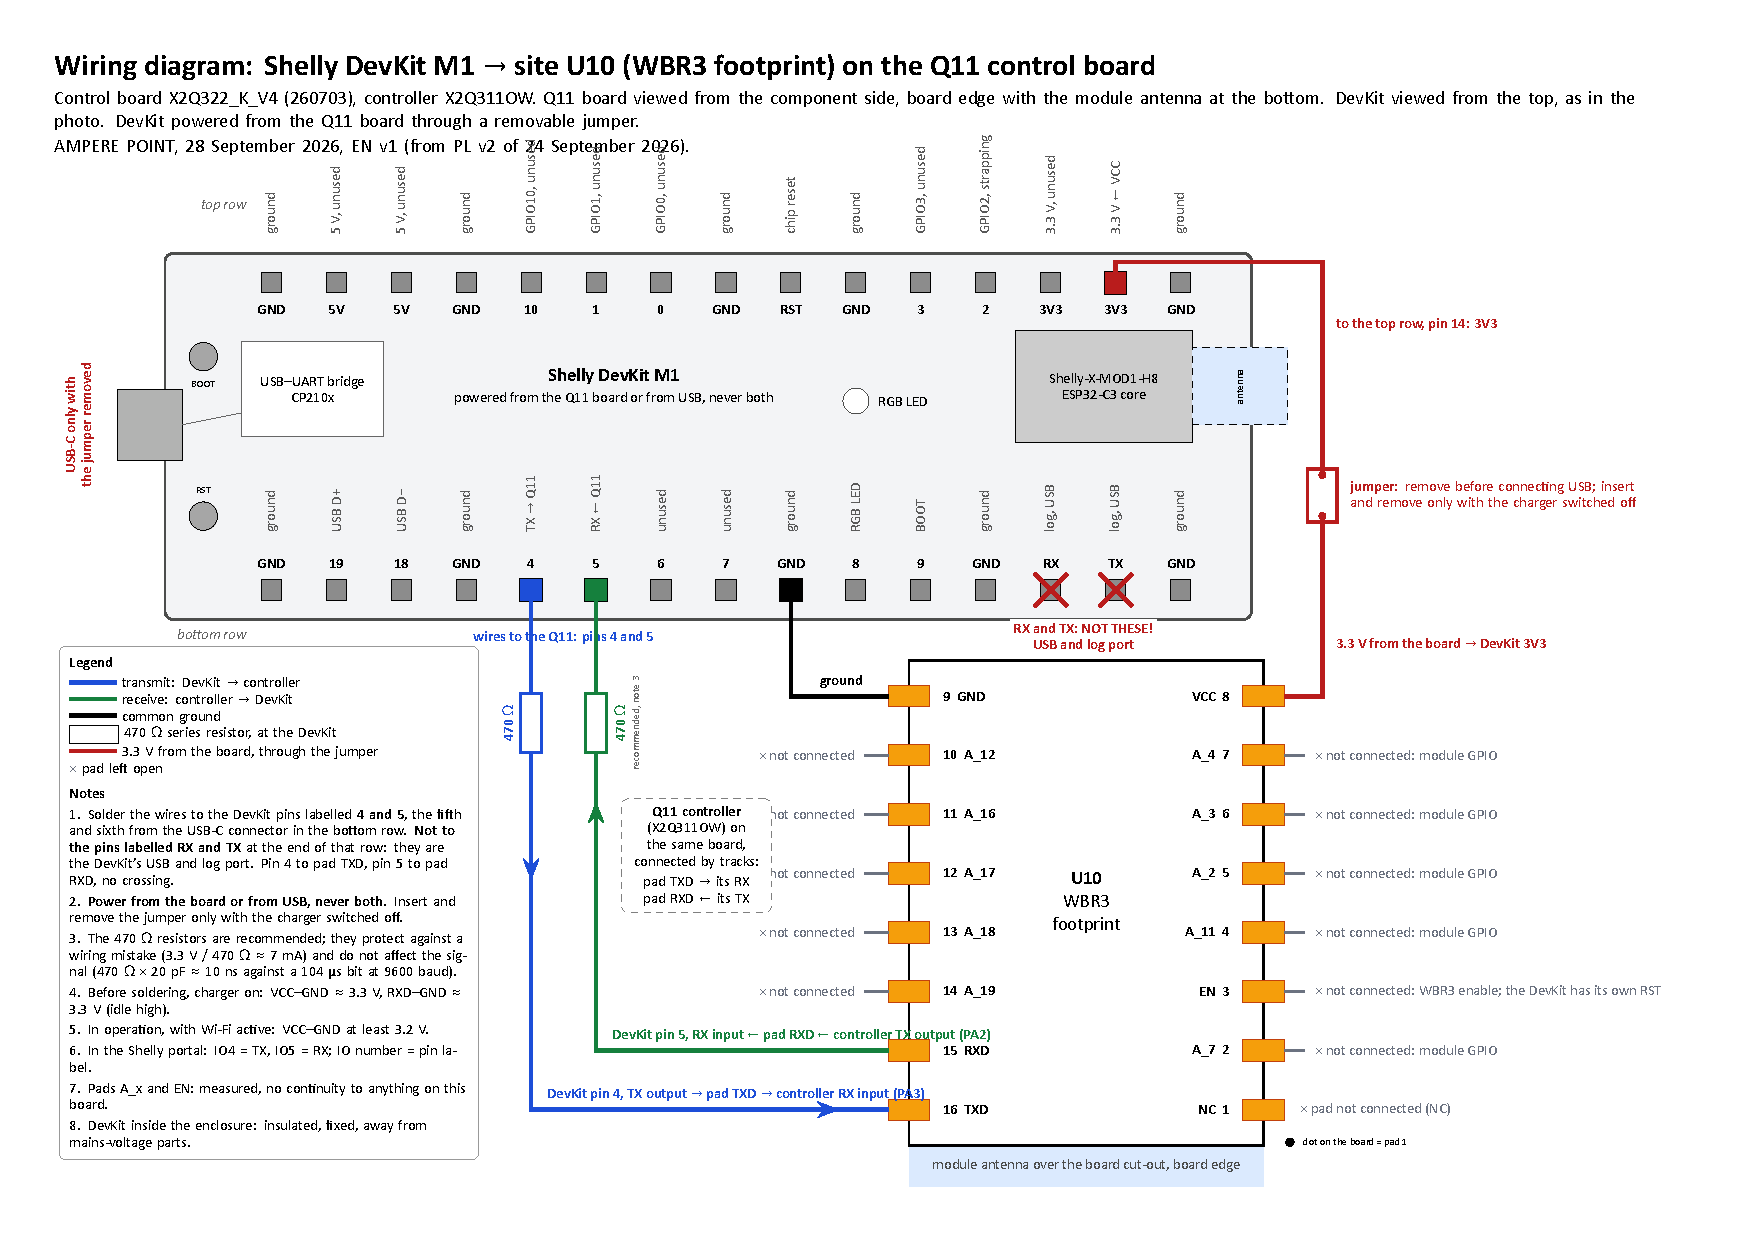
\includegraphics[width=\textwidth]{schematic_wiring_DevKit_Q11_EN.pdf}
\caption{Połączenia prototypu (pełnowymiarowy PDF w załączniku, strona 2 pokazuje każde pole U10; rysunek po angielsku).}
\label{fig:wiring}
\end{figure}

\begin{figure}[H]
\centering
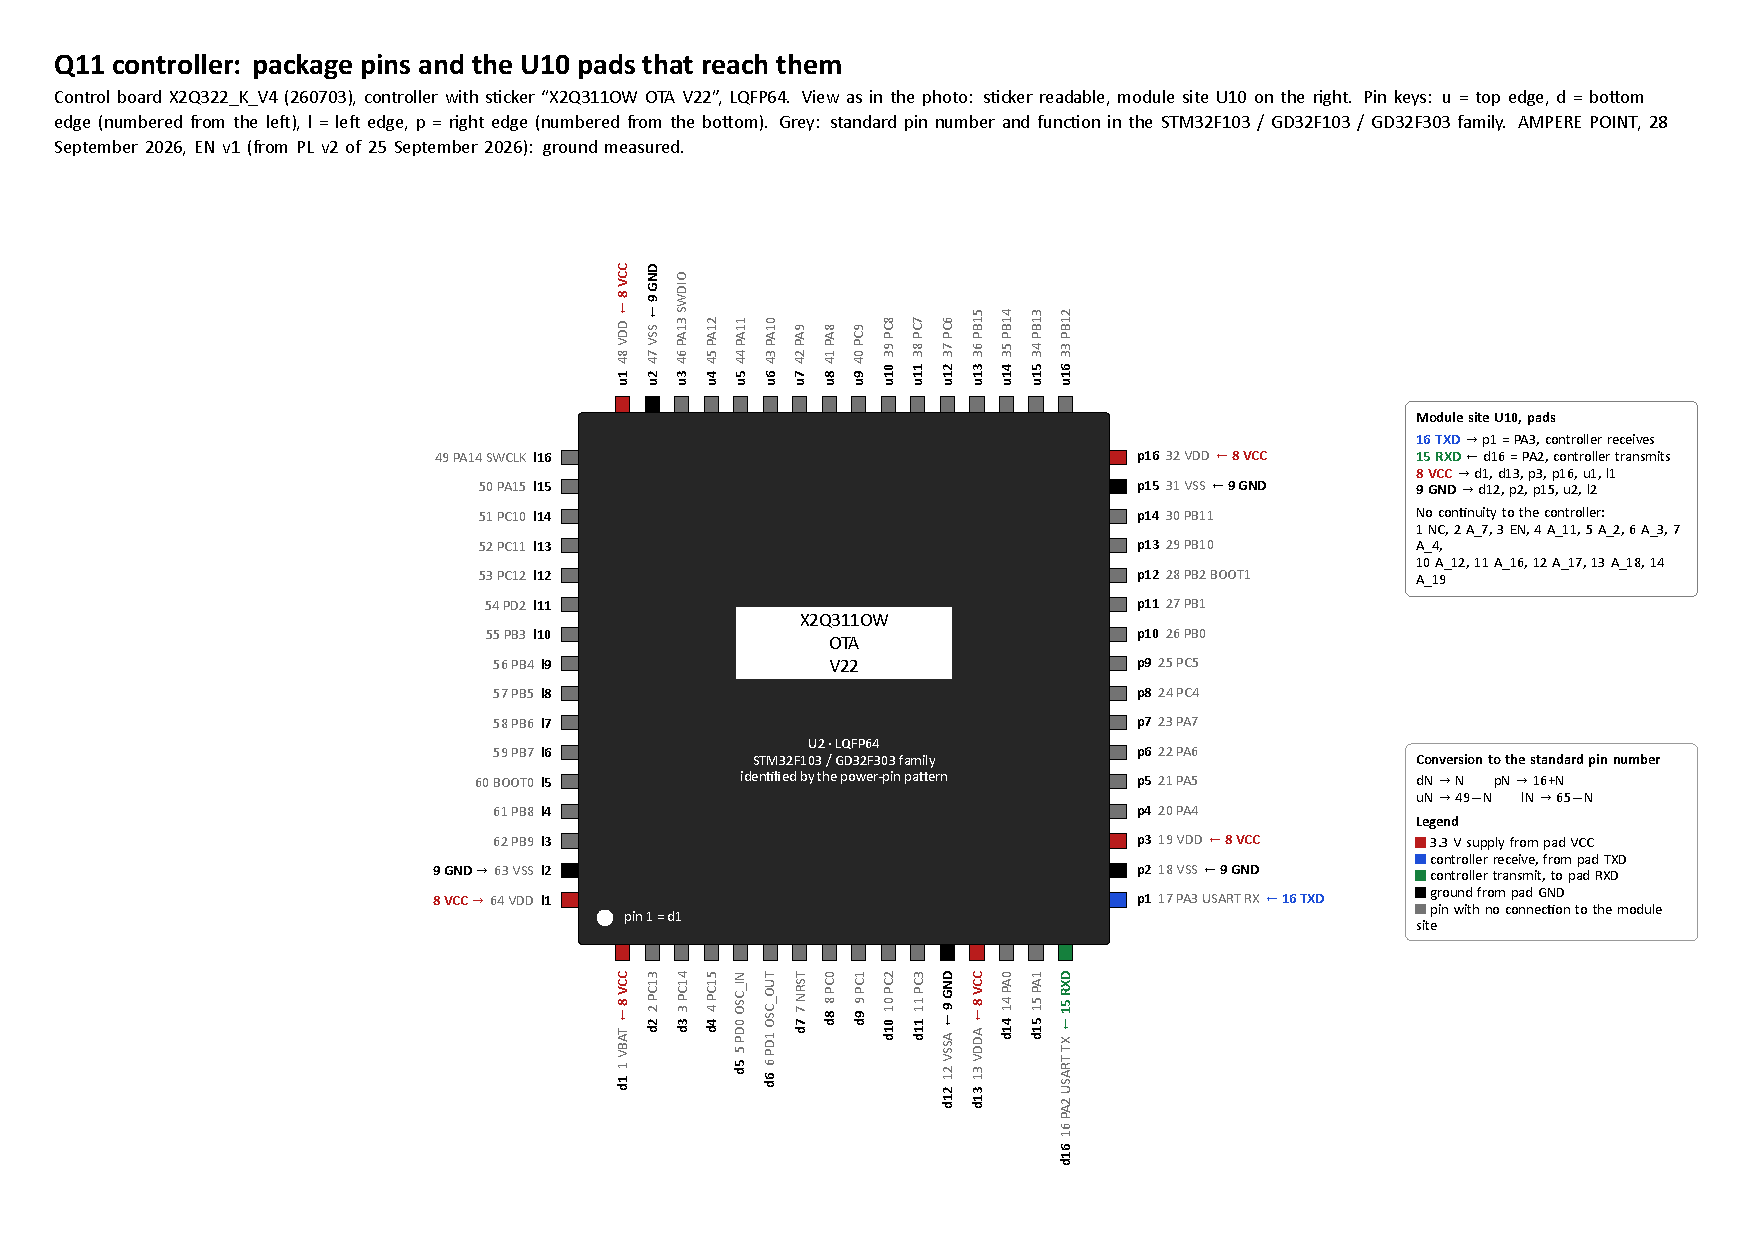
\includegraphics[width=\textwidth]{schematic_Q11_MCU_pins_EN.pdf}
\caption{Nóżki sterownika z polami U10, które do nich docierają (pełnowymiarowy PDF w załączniku; rysunek po angielsku).}
\label{fig:mcu}
\end{figure}

\section{Protokół szeregowy zaobserwowany na przewodzie}

\subsection{Warstwa fizyczna i format ramki}

9600~b/s, 8 bitów danych, bez parzystości, 1 bit stopu, poziomy 3,3~V. Protokół szeregowy Tuya MCU: \hx{55 AA} $|$ wersja $|$ polecenie $|$ długość (2 bajty, starszy pierwszy) $|$ dane $|$ suma kontrolna (suma wszystkich poprzednich bajtów modulo 256). Sterownik wysyła wersję \hx{03}; moduł wysyła wersję \hx{00}. Oprogramowanie Shelly ma ten protokół wbudowany (składnik „Tuya MCU”); AmperePoint nie napisał żadnego kodu protokołu.

\subsection{Sekwencja startowa}

Zarejestrowana 25 września 2026 o 11:51, gdy moduł inicjował się ponownie po wgraniu konfiguracji (sterownik pozostał zasilony):

\begin{longtable}{>{\raggedright\arraybackslash}p{1.6cm}>{\raggedright\arraybackslash}p{2.3cm}>{\raggedright\arraybackslash}p{4.1cm}>{\raggedright\arraybackslash}p{7.7cm}}
\toprule
\rowcolor{aphead}\textbf{Czas} & \textbf{Kierunek} & \textbf{Ramka (polecenie, dane)} & \textbf{Znaczenie} \\
\midrule\endhead
\bottomrule\endfoot
11:51:08 & sterownik \ra\ moduł & \hx{0x24} & sterownik pyta o siłę sygnału Wi-Fi \\
11:51:08 & moduł \ra\ sterownik & \hx{0x24 [C7]} & odpowiedź: $-57$~dBm \\
11:51:09 & moduł \ra\ sterownik & \hx{0x00} & znak życia \\
11:51:09 & sterownik \ra\ moduł & \hx{0x00 [01]} & odpowiedź na znak życia, \hx{01} = sterownik już pracuje (nie świeży start) \\
11:51:14 & moduł \ra\ sterownik & \hx{0x03 [04]} & stan Wi-Fi 4 (w pojęciach Tuya: połączony z chmurą) \\
11:51:14 & sterownik \ra\ moduł & \hx{0x03} & potwierdzenie \\
11:51:14 & moduł \ra\ sterownik & \hx{0x08} & zapytanie o wszystkie punkty danych \\
11:51:16--17 & sterownik \ra\ moduł & 12 $\times$ \hx{0x07} & meldunki punktów danych, w kolejności: 3, 4, 6, 7, 8, 9, 10, 14, 18, 19, 24, 13 \\
11:51:16 & sterownik \ra\ moduł & \hx{0x1C} & sterownik pyta o czas \\
11:51:17 & moduł \ra\ sterownik & \hx{0x1C [01 1A 09 19 0B 33 12 05]} & ważny, 2026-09-25 11:51:18, dzień tygodnia 5 \\
\end{longtable}

Wymiana informacji o produkcie (polecenia \hx{0x01} i \hx{0x02}) odbywa się, zanim dziennik diagnostyczny jest osiągalny przez Wi-Fi, i nie została zarejestrowana; patrz pytanie~2.

\subsection{Ruch rutynowy}

\begin{itemize}
\item Moduł \ra\ sterownik: znak życia \hx{0x00} co 15~s; stan Wi-Fi \hx{0x03 [04]} co 30~s. Sterownik odpowiada na oba.
\item Sterownik \ra\ moduł: pytanie o czas \hx{0x1C} i o siłę sygnału \hx{0x24}, każde w nieregularnych odstępach około 10--45~s. Moduł odpowiada na pytanie o czas dopiero po zsynchronizowaniu zegara (NTP); wcześniej wysyła \hx{01 00 00 00 00 00 00 00} (flaga „ważny” z zerową datą). Dlatego przy pracy ładowarki bez internetu AmperePoint dostarcza lokalny serwer NTP.
\item Sterownik \ra\ moduł, samoistne meldunki \hx{0x07}: temperatura (DP~24) przy każdej zmianie, stan połączenia (DP~13) przy każdej zmianie stanu sygnału do auta, limit prądu (DP~4) i włącznik (DP~18) po każdym zapisie, energia sesji (DP~25) raz na koniec sesji.
\end{itemize}

\subsection{Zachowanie przy zapisie}

Przy zapisie (\hx{0x06}) sterownik najpierw melduje \textbf{starą} wartość, a około sekundę później \textbf{nową}. Przykład, limit prądu 12~A \ra\ 10~A, 25 września 2026:

\begin{longtable}{>{\raggedright\arraybackslash}p{1.6cm}>{\raggedright\arraybackslash}p{2.5cm}>{\raggedright\arraybackslash}p{6.3cm}>{\raggedright\arraybackslash}p{5.4cm}}
\toprule
\rowcolor{aphead}\textbf{Czas} & \textbf{Kierunek} & \textbf{Pełna ramka} & \textbf{Znaczenie} \\
\midrule\endhead
\bottomrule\endfoot
11:56:48 & moduł \ra\ sterownik & \hx{55 AA 00 06 00 08 04 02 00 04 00 00 00 0A 21} & ustaw DP~4 (typ liczbowy, 4 bajty) = 10 \\
11:56:49 & sterownik \ra\ moduł & \hx{55 AA 03 07 00 08 04 02 00 04 00 00 00 0C 27} & meldunek DP~4 = 12 (jeszcze stara wartość) \\
11:56:50 & sterownik \ra\ moduł & \hx{55 AA 03 07 00 08 04 02 00 04 00 00 00 0A 25} & meldunek DP~4 = 10 (przyjęte) \\
10:52:37 & moduł \ra\ sterownik & \hx{55 AA 00 06 00 05 12 01 00 01 01 1F} & ustaw DP~18 (logiczny) = 1, ładowanie włączone \\
10:52:38 & sterownik \ra\ moduł & \hx{55 AA 03 07 00 05 12 01 00 01 01 23} & meldunek DP~18 = 1 \\
-- & sterownik \ra\ moduł & \hx{55 AA 03 00 00 01 01 04} & odpowiedź na znak życia, dla porównania \\
\end{longtable}

Wartości 8, 10, 12, 14 i 16~A zostały zapisane i potwierdzone przez sterownik w ten sam sposób.

\section{Punkty danych}

\subsection{Trzy warstwy}

Sterownik wysyła meldunki punktów danych na przewód niezależnie od tego, jaki moduł słucha; moduł Shelly odbiera każdą ramkę dokładnie tak, jak odbierał ją WBR3. Różnica leży w tym, gdzie jest zdefiniowane znaczenie punktu danych: przy WBR3 to definicja produktu w chmurze Tuya, przy module Shelly to konfiguracja produktu napisana przez AmperePoint. Log potwierdza, że moduł Shelly rejestruje każdy zgłoszony punkt danych, także niezadeklarowany w konfiguracji produktu (wpisy w logu takie jak \texttt{add int 24}, \texttt{add enum 13}, \texttt{add raw 19}).

\begin{longtable}{>{\raggedright\arraybackslash}p{6.2cm}>{\raggedright\arraybackslash}p{3.0cm}>{\raggedright\arraybackslash}p{6.9cm}}
\toprule
\rowcolor{aphead}\textbf{Warstwa} & \textbf{Punkty danych} & \textbf{Kto definiuje} \\
\midrule\endhead
\bottomrule\endfoot
Odebrane i zapamiętane przez moduł & wszystkie, które sterownik wysyła: zaobserwowano 13 różnych numerów & oprogramowanie sterownika \\
Zadeklarowane w produkcie Shelly, dostępne dla skryptu usługi & 7 (1, 3, 4, 6, 7, 8, 18) & AmperePoint, w portalu \\
Pokazane jako pola (aplikacja, lokalne API, MQTT) & 6 pól & AmperePoint, w skrypcie usługi \\
\end{longtable}

Wyliczenia idą po przewodzie jako bajt indeksu; nazwy istnieją tylko w definicji produktu. Produkt Shelly używa tej samej kolejności co definicja Tuya (pytanie~7 prosi o potwierdzenie).

\subsection{Porównanie: definicja produktu Tuya, zachowanie sterownika, produkt Shelly}

Definicja z produktu Tuya \emph{Ampere Point Q11 PRO} (17 punktów danych). „Zgłaszany” = widziany w logu modułu 25 września 2026: \textbf{zrzut} = w odpowiedzi na zapytanie \hx{0x08}, \textbf{samoist.} = wysłany przez sterownik z własnej inicjatywy, \textbf{nigdy} = nie widziany w żadnej ramce.

\begin{longtable}{>{\raggedright\arraybackslash}p{0.7cm}>{\raggedright\arraybackslash}p{3.1cm}>{\raggedright\arraybackslash}p{3.6cm}>{\raggedright\arraybackslash}p{0.9cm}>{\raggedright\arraybackslash}p{3.2cm}>{\raggedright\arraybackslash}p{3.8cm}}
\toprule
\rowcolor{aphead}\textbf{DP} & \textbf{Kod Tuya} & \textbf{Typ, jednostka, kodowanie} & \textbf{R/W} & \textbf{Zgłaszany przez sterownik} & \textbf{W produkcie Shelly} \\
\midrule\endhead
\bottomrule\endfoot
1 & forward\_\allowbreak energy\_\allowbreak total & liczba, kWh, skala 2 (\hx{123456} = 1234,56~kWh) & R & \no\ nigdy (ani w zrzucie, ani samoist.) & zadeklarowany, przeznaczony na licznik całkowity; zostaje 0, bo nic nie przychodzi. Pytanie~4 \\
3 & work\_state & wyliczenie, 8 stanów: 0 free, 1 insert, 2 free\_fault, 3 wait, 4 charging, 5 pause, 6 end, 7 fault & R & \ok\ zrzut; widziane wartości 0 i 3 & \ok\ pole „mode”, indeks tłumaczony na nazwę \\
4 & charge\_cur\_set & liczba, A, 6--32 & RW & \ok\ zrzut; zapisy 8/10/12/14/16 potwierdzone & \ok\ pole „current limit”, ograniczone do 6--16~A dla Q11 \\
6, 7, 8 & phase\_a / b / c & surowe, 7 bajtów: napięcie 2~B $\times$0,1~V, prąd 3~B $\times$0,001~A, moc 2~B w W & R & \ok\ zrzut; 226--228~V przy zamkniętym styczniku; prąd i moc jeszcze nie widziane pod obciążeniem & \ok\ dekodowane w skrypcie do pola „phase info” \\
9 & power\_total & liczba, kW, skala 3 & R & \ok\ zrzut; 0 & \half\ skrypt sumuje fazy zamiast tego \\
10 & fault & mapa bitowa, 17 bitów: ov\_cr, ov2\_cr\_fault, ov\_vol, undervoltage\_alarm, contactor\_adhesion, contactor\_fault, earth\_fault, meter\_hardware\_alarm, scram\_fault, cp\_fault, meter\_commu\_fault, card\_reader\_fault, cir\_short\_fault, adhesion\_fault, self\_test\_alarm, leakagecurr\_alarm, ov\_Temp\_fault & R & \ok\ zrzut; 0 & \half\ odbierany, jeszcze nie pokazany jako pole \\
13 & connection\_state & wyliczenie, 7: 0 12V, 1 12V\_pwm, 2 9V, 3 9V\_pwm, 4 6V, 5 6V\_pwm, 6 error & R & \ok\ zrzut + samoist.; widziane wartości 0, 2, 4 & \half\ odbierany, jeszcze nie pokazany \\
14 & work\_mode & wyliczenie, 3: 0 charge\_now, 1 charge\_energy, 2 charge\_schedule & RW & \ok\ zrzut; 0 & \half\ odbierany, jeszcze nie pokazany \\
17 & energy\_charge & liczba, kWh, 1--200 & RW & \no\ nigdy & niezadeklarowany. Pytanie~4 \\
18 & switch & logiczny & RW & \ok\ zrzut + samoist. po zapisie & \ok\ pole „state” \\
19 & local\_timer & surowe, 2 bajty: godzina startu, godzina końca & RW & \ok\ zrzut; \hx{00 00} & \half\ odbierany, jeszcze nie pokazany \\
23 & system\_version & tekst & R & \no\ nigdy & niezadeklarowany. Pytanie~4 \\
24 & temp\_current & liczba, °C, $-40$--200 & R & \ok\ zrzut + samoist. przy zmianie; 18--20~°C & \half\ odbierany, jeszcze nie pokazany \\
25 & charge\_\allowbreak energy\_\allowbreak once & liczba, kWh, skala 2 & R & \half\ raz: wartość 0, w jednej ramce z DP~18 = 0 & \half\ energia sesji jest dziś liczona w skrypcie; przejdzie na DP~25 \\
33 & mode\_set & surowe & RW & \no\ nigdy & niezadeklarowany. Pytanie~5 \\
\end{longtable}

Zrzut w odpowiedzi na \hx{0x08} zawiera 12 punktów danych w kolejności: 3, 4, 6, 7, 8, 9, 10, 14, 18, 19, 24, 13. Punktów 1, 17, 23 i 33 nie ma w zrzucie i nigdy nie zostały wysłane samoistnie.

\section{Wyniki testów}

\begin{longtable}{>{\raggedright\arraybackslash}p{4.2cm}>{\raggedright\arraybackslash}p{1.7cm}>{\raggedright\arraybackslash}p{10.1cm}}
\toprule
\rowcolor{aphead}\textbf{Test} & \textbf{Wynik} & \textbf{Szczegóły} \\
\midrule\endhead
\bottomrule\endfoot
Komunikacja ze sterownikiem & \ok & protokół Tuya MCU, 9600 8N1; odpowiedzi na znak życia; meldunki punktów danych; bez zmian w oprogramowaniu sterownika \\
Pola używane przez płytkę & \ok & tylko VCC, GND, RXD, TXD; dwanaście pól wolnych \\
Zasilanie modułu z płytki & \ok & 3,3~V ze stabilizatora płytki; bez spadków napięcia w czasie prób \\
Włączanie ładowania z modułu & \ok & zapis DP~18, potwierdzony przez sterownik w ciągu 1~s \\
Limit prądu z modułu & \ok & 8, 10, 12, 14, 16~A zapisane i potwierdzone \\
Odczyt stanu & \ok & stan pracy, stan połączenia, temperatura, bity błędów, tryb pracy, okno godzin, napięcia faz \\
Czas dostarczony sterownikowi & \ok & odpowiedź na \hx{0x1C} z poprawnym czasem lokalnym, gdy moduł ma NTP; w pracy bez internetu lokalny serwer NTP \\
Stan Wi-Fi dla sterownika & \ok & \hx{0x03 [04]} co 30~s; wyświetlacz ładowarki pokazuje ikonę sieci \\
Praca bez jakiejkolwiek chmury & \ok & chmura Shelly wyłączona; moduł sterowany przez sieć lokalną (HTTP, WebSocket, MQTT) i przez Bluetooth \\
Lokalna warstwa integracji & \ok & patrz niżej \\
Ładowanie pod obciążeniem & \half & użyto symulatora auta do stanów sygnału sterującego; pełna sesja z przepływem prądu jeszcze do zrobienia \\
Aktualizacja sterownika przez moduł & \no\ nie testowano & patrz pytanie~9 \\
Reset Wi-Fi z menu ładowarki & \no\ nie testowano & patrz pytanie~8 \\
\end{longtable}

\begin{apbox}[Lokalna warstwa integracji (middleware), dla informacji]
Moduł Shelly udostępnia lokalne API (HTTP, WebSocket, MQTT). Na nim AmperePoint uruchamia niewielką warstwę oprogramowania poza ładowarką: broker MQTT, lokalny serwer NTP oraz most, który przedstawia Q11 systemowi ładowania jako punkt ładowania OCPP~1.6J (rejestracja, stan, zdalny start, limit prądu przez profil ładowania, odczyty licznika). Wszystko to sprawdzono z lokalnym serwerem testowym. Warstwa działa na komputerze albo serwerze, nie w ładowarce, i \textbf{nie wymaga niczego od oprogramowania sterownika}. Wspomniana jest tu tylko po to, żeby widać było całość.
\end{apbox}

\section{Pytania otwarte do producenta}

\begin{enumerate}
\item \textbf{Oznaczenie sterownika.} Jaki mikrokontroler jest pod naklejką „X2Q311OW OTA V22” (STM32F103xx, GD32F103xx, GD32F303xx, inny) i jaki ma rozmiar pamięci flash?
\item \textbf{Ramka informacji o produkcie.} Co sterownik odpowiada na zapytanie o produkt (\hx{0x01}): klucz produktu \texttt{p}, wersja oprogramowania \texttt{v}, tryb pracy modułu \texttt{m}? Którą wersję Tuya MCU SDK / protokołu realizuje oprogramowanie? Nie mogliśmy zarejestrować tej wymiany, bo odbywa się, zanim dziennik modułu jest osiągalny.
\item \textbf{Pola niepodłączone.} Dwanaście pól U10 (NC, A\_7, EN, A\_11, A\_2, A\_3, A\_4, A\_12, A\_16, A\_17, A\_18, A\_19) nie ma ciągłości z niczym. Prosimy o potwierdzenie na podstawie schematu, że płytka używa tylko VCC, GND, RXD i TXD modułu i że oprogramowanie nie oczekuje żadnego sygnału na pozostałych polach (na przykład EN albo linii resetu).
\item \textbf{Punkty danych nigdy niezgłaszane.} DP~1 (forward\_energy\_total), DP~17 (energy\_charge), DP~23 (system\_version) i DP~33 (mode\_set) nie były w zrzucie i nigdy nie zostały wysłane samoistnie. W jakich warunkach sterownik zgłasza każdy z nich? DP~25 (charge\_energy\_once) został wysłany raz, z wartością 0, razem z DP~18 = 0: czy to meldunek końca sesji?
\item \textbf{DP~33 mode\_set.} Jaki jest format bajtów i znaczenie tego surowego punktu danych?
\item \textbf{DP~8.} W eksporcie \texttt{Q21\_11kW\_with\_OTA} DP~8 nazywa się \texttt{charger\_events}, w definicji \emph{Q11 PRO} to \texttt{phase\_c}. Nasz egzemplarz wysyła DP~8 jako 7-bajtową wartość surową w tym samym formacie co DP~6 i DP~7. Której definicji trzyma się wysyłane oprogramowanie i czy format różni się między wersjami?
\item \textbf{Kolejność wyliczeń.} Prosimy o potwierdzenie kolejności indeksów DP~3, DP~13 i DP~14 według tabeli wyżej.
\item \textbf{Stan Wi-Fi i parowanie.} Których wartości stanu Wi-Fi (\hx{0x03}, 0--7) używa sterownik i do czego (ikona na wyświetlaczu, zachowanie)? Co pozycja menu ładowarki do resetu sieci / parowania wysyła do modułu (\hx{0x04} czy \hx{0x05})?
\item \textbf{Aktualizacja sterownika przez moduł.} Czy sterownik obsługuje polecenia aktualizacji Tuya MCU (\hx{0x0A} start, \hx{0x0B} przesyłanie pakietów)? W jakim formacie plik trafia na platformę Tuya do OTA sterownika (zwykły plik binarny?) i czy ten sam plik może zostać przekazany AmperePoint, żeby moduł Shelly, który realizuje te same polecenia aktualizacji, mógł aktualizować sterownik? Czy program rozruchowy toleruje przerwaną aktualizację?
\item \textbf{Czas.} Sterownik pyta o czas (\hx{0x1C}) co 10--45~s. Do czego używa czasu (okno godzin DP~19, wyświetlacz, zapisy sesji) i co się dzieje, gdy moduł nigdy nie dostarczy ważnego czasu?
\item \textbf{Zachowanie przy milczącym module.} Sterownik pracował normalnie, gdy moduł przez dzień nic nie wysyłał (źle podłączony prototyp). Czy jest jakiś limit czasu na znak życia albo na stan Wi-Fi, który zmienia zachowanie sterownika?
\end{enumerate}

\section{Załączniki}

\begin{itemize}
\item \texttt{ShellyX\_module\_X1\_datasheet\_v14.pdf}: karta katalogowa modułu docelowego (Shelly).
\item \texttt{schematic\_wiring\_DevKit\_Q11\_EN.pdf}: połączenia prototypu i funkcja każdego pola U10 (po angielsku).
\item \texttt{schematic\_Q11\_MCU\_pins\_EN.pdf}: nóżki sterownika z polami U10, które do nich docierają (po angielsku).
\item Logi modułu na poziomie ramek (25 września 2026) dostępne na życzenie.
\end{itemize}

{\color{apmuted}\small AMPERE POINT — R\&D · www.amperepoint.pl · Opracowano 28 września 2026 na podstawie pomiarów na egzemplarzu Q11, dziennika diagnostycznego modułu i definicji produktów Tuya.}

\end{document}
